\pagebreak
\subsection{Electrical Design}
The electrical design provided the hardware required for the implementation of the software, the sensors for the control system and furthermore a communication interface to the BEXUS system. A global diagram with the electrical interfaces between the IRISC experiment and BEXUS balloon is shown in figure \ref{fig:elec-ACD}. %The main interfaces are the E-Link and the power. But also, the camera's/ telescope should be able to watch the sky from the gondola.}}
\vspace{-.5cm}
\begin{figure}[H]
	\centering
	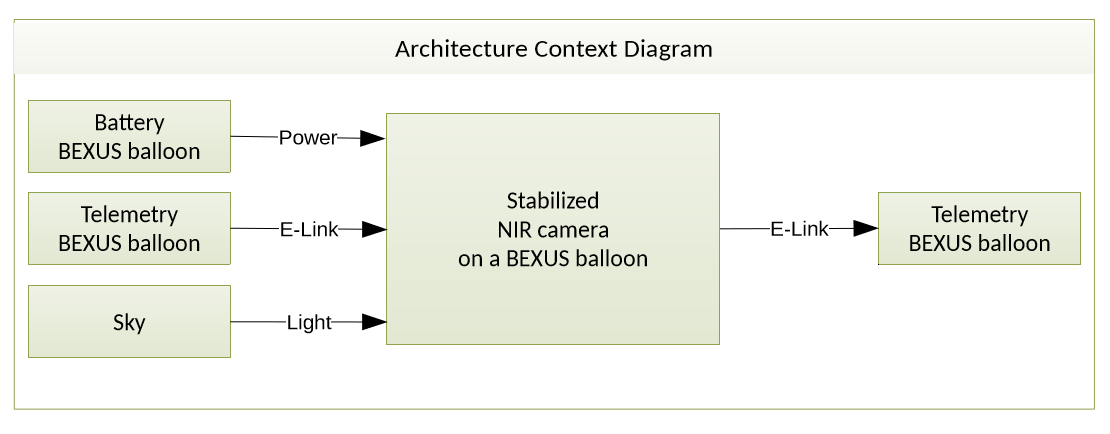
\includegraphics[width=.6\textwidth]{4-experiment-design/img/electrical/ArchitectureContext.png}
	\caption{Electrical architecture context diagram.}
	\label{fig:elec-ACD}
\end{figure}


\subsubsection{Block Diagram}
\label{sec:4.5.1}
The architecture interconnect diagram of the electrical design is shown in figure \ref{fig:elec-AID}. The main controller was the Raspberry Pi. There was external storage for the obtained images. To stabilize the pictures the gyroscopes (relative) and encoders (absolute) were used. This would give enough information to stabilize the camera during one picture (accuracy $<$ 0.5 arcseconds required to achieve requirement P.8). Because the gondola also moved, a star tracker and GPS were used to measure this. Potentionally, an accelerometer and a compass would be used for additional complementary data. These only had to be accurate enough to have the target in the field of view of the camera ($<$ 0.5 degrees for the star tracker (P.9), $<$ 5 meters for the GPS (P.10)).
\vspace{-.5cm}
\begin{figure}[H]
	\centering
	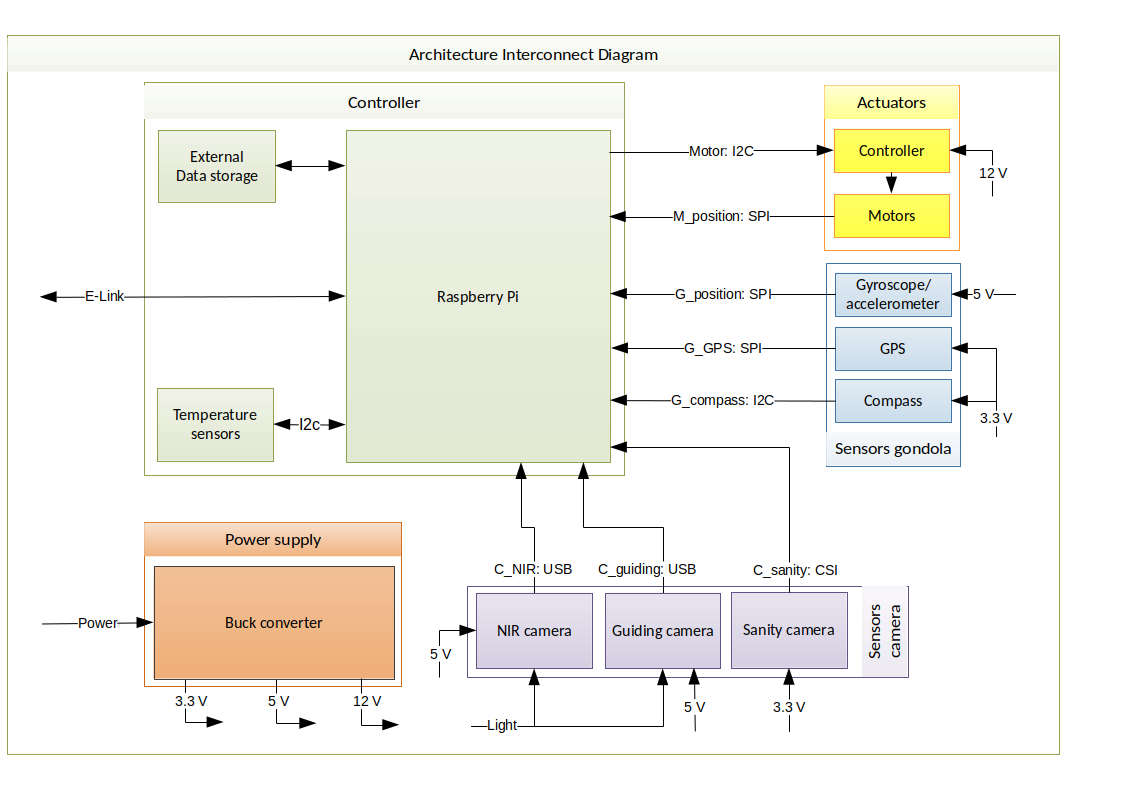
\includegraphics[width=.85\textwidth]{4-experiment-design/img/electrical/ArchitectureInterconnect.png}
	\caption{Electrical architecture interconnect diagram.}
	\label{fig:elec-AID}
\end{figure}

\subsubsection{Motor-controller \& Motor}
{The motor has been changed to a stepper motor. But due to the lack of which stepper, the electrical circuit has not been made yet. There are multiple microstep controllers that could be used. The stepper has to be able to rotate the telescope with a speed of 700\,arcseconds per second, with an accuracy of atleast 1 arcsecond. The main problem at this stage is that the electrical team does not know how much force is needed before the gears including the lose. The "SM-42BYG011-25" stepper, which was our first option, will probably not be able to met all these requirements.\\

Depending on the amount of microsteps needed, the controller will be chosen as soon as the final stepper is defined. The output of the controller will then be amplified by voltage and current through a H-bridge.

\subsubsection{Encoders}
The chosen absolute encoder is an AMT23 with $2^{14}$ positions. One is located directly at the output of the stepper and the other one after the gearbox. Due to this a high accuracy (at least 0.25 arcseconds) can be achieved, while also be able to determine the exact position of the telescope, relative to the gondola. Since the encoders are absolute encoders and measure independently of the OBC, a watchdog reboot will not affect these measurements.\\

The chosen encoders has been tested and work as expected.


\subsubsection{IMU}
The chosen IMU was the STIM300 from sensonor. Consists of 3 axis gyroscope, 3 axis inclinometer and 3 axis accelerometer.

\subsubsection{GPS}
With the GPS the location and altitude can be determined. This is done with the uBlox NEO M8N. The accuracy is within 1.5 meters, which is within the requirements. A small error will not give a completely different night sky, thus this is enough for this application. The chosen GPS has been tested and work as expected.

\subsubsection{Connectors and cables}
The PCB has CLIK-MATE MOLEX connectors for the data signals going through a cable harness to D-SUB connectors on the outside of the electronics box. Except for Ethernet, which will be connected through a normal Ethernet connector. The camera's are connected to the USB, which will be mechanically locked into place. The interface to the outside will be done with a D-SUB connectors. The power cables will be in a separate cable harness to the outside of the electronics box. Here two power input connectors are located, in order to switch easily between power supplies. The cables towards the steppers are in the same cable harness, but will be connected to the outside with power D-SUB connectors. Almost all external components have cables directly connected to it without connectors, except for the encoders, these are connected with CLIK-MATE MOLEX connectors.

%\subsubsection{Star tracker}
%TODO : ADD THIS DECRIPTION
%\colorbox{yellow}{\parbox{\textwidth}{}}

\subsubsection{Schematic}
See Appendix c.

\subsubsection{PCB Layout}
One four layer PCB that controls everything, with dimensions 28cmx18cm, is placed inside the electronics box. 

\begin{figure}[H]
	\centering
	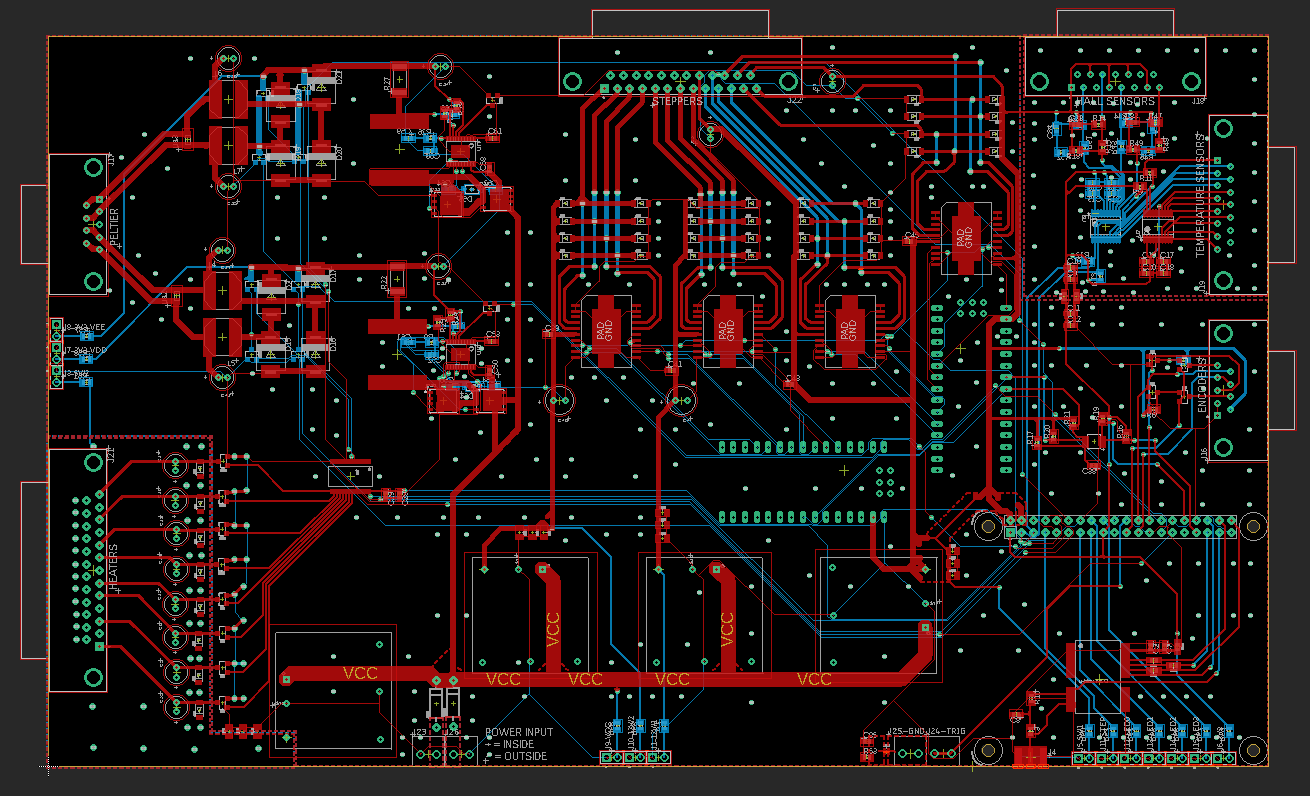
\includegraphics[scale=0.5]{4-experiment-design/img/electrical/PCBdesign.png}
	\caption{PCB design}
	\label{fig:electronic-box}
\end{figure}

\raggedbottom
